%% amssamp1.tex is nearly identical to amssamp2.tex, except
%% that amssamp2.tex uses the [twocol] option to produce
%% two-column text.

%\documentclass{ametsoc}

\documentclass[twocol]{ametsoc}

%%%%%%%%%%%%%%%%%%%%%%%%%%%%%%%%
%%% To be entered only if twocol option is used

\journal{jtech}
\usepackage{graphicx}
\usepackage{caption}
\usepackage{subcaption}
\usepackage{hyperref}
\usepackage{url}
%  Please choose a journal abbreviation to use above from the following list:
% 
%   jamc     (Journal of Applied Meteorology and Climatology)
%   jtech     (Journal of Atmospheric and Oceanic Technology)
%   jhm      (Journal of Hydrometeorology)
%   jpo     (Journal of Physical Oceanography)
%   jas      (Journal of Atmospheric Sciences)	
%   jcli      (Journal of Climate)
%   mwr      (Monthly Weather Review)
%   wcas      (Weather, Climate, and Society)
%   waf       (Weather and Forecasting)
%   bams (Bulletin of the American Meteorological Society)
%   ei    (Earth Interactions)

%%%%%%%%%%%%%%%%%%%%%%%%%%%%%%%%
%Citations should be of the form ``author year''  not ``author, year''
\bibpunct{(}{)}{;}{a}{}{,}

%%%%%%%%%%%%%%%%%%%%%%%%%%%%%%%%

\title{A report on progress on Corrected Moments in Antenna Coordinates 2.0}

\authors{Scott Collis\correspondingauthor{Scott Collis, Argonne National Laboratory, 
Environmental Science division, 
9700 South Cass Ave, Argonne, IL 60514} 
and Jonathan Helmus}

\affiliation{Environmental Science Division, Argonne National Laboratory} 

\email{scollis@anl.gov}

%\extraauthor{Extra Author}
%\extraaffil{Affiliation, City, State/Province, Country}



\abstract{In 2010 the Atmospheric Radiation Measurement program procured a number of 3 and 5cm wavelength radars for documenting the macrophysical, microphysical and dynamical structure of precipitating systems. In order to maximize the scientific impact the program supported the development of an application chain to correct for various phenomena in order to retrieve the "point" values of moments of the radar spectrum and polarimetric measurements. This report details the motivation, science and progress to date as well as charting a path forward.}

\begin{document}

\maketitle


\section{Introduction}
\label{sec:intro}
The Atmospheric Radiation Measurement Program (\cite{mather_arm_2012}) (ARM) has a long history of sensing clouds in the column using the Millimeter 
Cloud Radar (MMCR, Now Ka-Band Zenith Radar or KaZR). Starting in 2010 ARM embarked on program to better characterize the domain surrounding the 
column using scanning radars at millimeter and centimeter wavelengths. Processing for the shorter wavelengths has been previously published  \cite{kollias_scanning_2013} 
this report is limited to 5 and 3cm wavelengths. Due to the agility and lower cost per radar the program opted not to operate the common wavelength of 
10cm (S-Band) which is  robust to liquid water path attenuation in all but the most severe storms. This necessitates the development of robust code for the 
correction of issues due to the two way propagation of the radar through medium that both scatters and attenuates. In addition, the trade off between wavelength, 
maximum unambiguous range and Doppler nyquist velocity means the radars alias at 12.4 and 16.52 $\mathrm{ms^{-1}}$ for 3 and 5cm respectively when 
operating in a baseline mode (such as during the Mid-Latitude  Convective Continental Clouds Experiment $\mathrm{MC^3E} $ (\cite{jensen_midlatitude_2015}).
 Due to extreme velocities of scatterers aloft and, in places such as Oklahoma, at the surface, aliasing is common and requires post moment calculation dealiasing. 
 There are many techniques for dealiasing Doppler velocities (eg \cite{james_real-time_2001}) however on testing we found these techniques to be either 
 difficult to implement in an operational chain or lacking in robustness. 

When we first attempted to build a processing chain each step made its own decision on where to conditionally run based on various measurements
 of "quality"  such as the co-polar (zero lag) correlation coefficient $\mathrm{\rho_{HV}}$ and Normalized Coherent Power (NCP, also referred to as 
 Signal Quality Index or SQI). These are defined as:
\begin{align}
\rho_{HV}(0) &= \frac{|<S_{VV}S_{hh}^*>|}{\sqrt{<|S_{HH}|^2><|S_{VV}|^2>}}\\
NCP &= \frac{P_{coh}}{P_{DC}}.
\end{align}

Where the $S$ terms are elements of the scattering matrix, $P_{coh}$ is the coherent part of the doppler spectrum and $P_{DC}$ is the incoherent part.
 Since ARM radars use magnetron transmitters the phase is randomized from pulse to pulse so when a first trip return is mixed with a return from a scatterer
  beyond the maximum unambiguous range the derived radar Doppler spectrum when averaged over many pulses is flat and the NCP is low. While the 
  Doppler spectrum from a first trip has structure from which (depending on the method) a peak can be found and Doppler velocity determined and the NCP
   approaches 1.0. However, the usefulness of NCP alone in second trip detection breaks down in regions of high spectral width. When the spectral width
    approaches the nyquist velocity, even in areas of purely first trip, the NCP decreases. This is especially troublesome in regions of high convergence 
    and divergence in convective storms, often causing false flagging of these regions. 

To overcome the issues of arbitrary decision making and faults in using NCP alone to detect multiple trips our application chain, Corrected Moments in
 Antenna Coordinates first attempts to identify the nature of the scattering medium at the gate. This gate-ID is performed before any corrections are
  applied so it is different to hydrometeor identification codes (eg \cite{dolan_theory-based_2009}, \cite{wen_cluster-based_2015}, \cite{al-sakka_new_2013} etc.) 
  that seek to gain microphysical insight. Gate-ID is performed for the purpose of objectively determining where future algorithms should be applied. 
  Since we are implementing CMAC2.0 using the Python-ARM Radar Toolkit (Py-ART, \cite{heistermann_emergence_2014}) we can use the the
   identifications to construct a \href{https://github.com/ARM-DOE/pyart/blob/master/pyart/filters/gatefilter.py#L111 }{gate filter}.


\section{Application chain}
There exists many algorithms in the scientific literature for the quality control and correction of radar data. Far to many to adequately 
asses and implement. However, given Py-ART's data model driven approach it is possible to design an application chain that is highly 
modular and task based. Each component has a particular job and can be replaced as better algorithms are published (and, ideally, code shared). 
As stated in the previous section, the overarching idea behind CMAC2.0 is a gate-ID is created and determines the conditional
 application of algorithms. At the time of writing implemented classes are: Rain, melting layer, ice, second trip and no significant 
 scatterer. Dealiasing, for example would run on the set of all classes except "no significant return" while retrievals of specific 
 attenuation would run on the class of "rain". This approach requires that the gate-ID is run on the pre-corrected data. However,
  as discussed in sec \ref{sec:intro}, radar provided measurements alone are not sufficient to constrain the problem of gate-ID, 
  especially the identification of multiple trips. There are a number of pre-ID retrievals and inputs we can generate to constrain
   the problem, however, and these are described in \ref{ssec:precalc}. 

The Application chain for CMAC2.0 is shown in fig ~\ref{fig:chain} and can be broken down to:
\begin{itemize}  
\item Pre-ID calculations of texture and mapping sounding data to radar gates
\item Ascribing membership functions to gate classes, scoring of gates and classification at the gate of predominate scatterer.
\item Dealiasing of Doppler velocities.
\item Extraction of propagation differential polarimetric phase from instrument measured differential polarimetric phase.
\item Calculation of specific differential phase.
\item Calculation of specific attenuation.
\item Integrate and apply to reflectivity.
\item Calculate rain rate for liquid precipitation using specific attenuation.
\end{itemize} 

\begin{figure}[h]
    \centering
    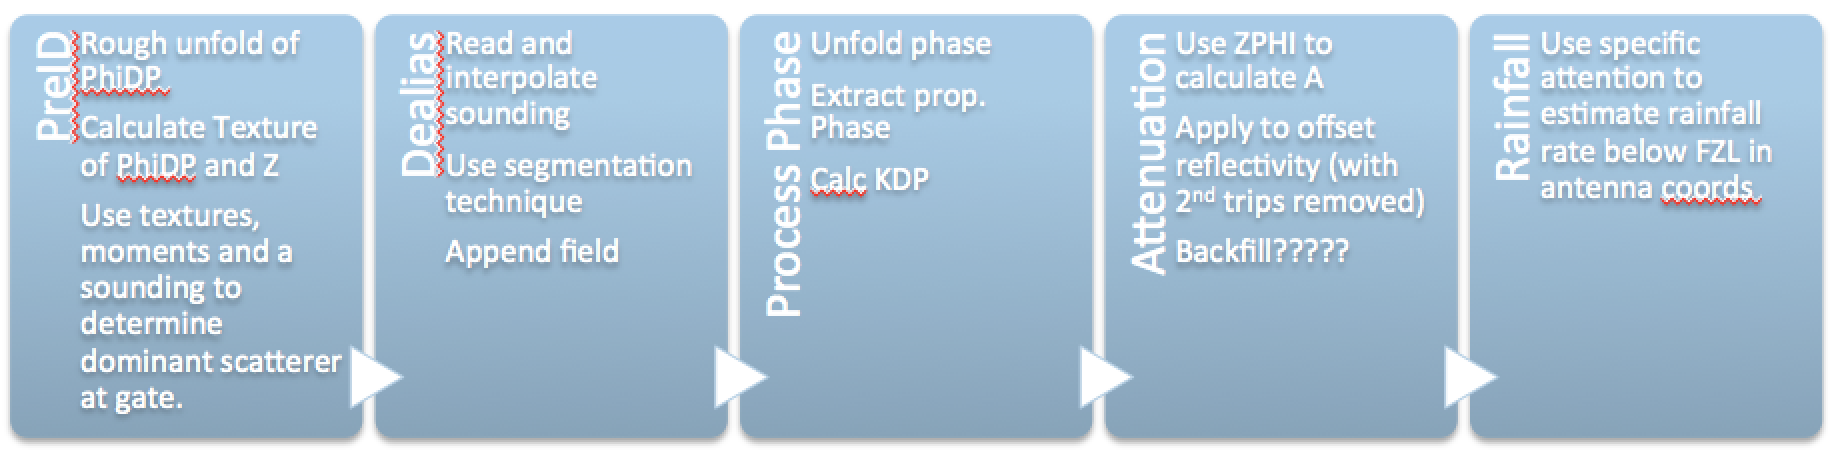
\includegraphics[width=0.9\columnwidth]{application_chain.png}
    \caption{The Application chain for Corrections in Antenna Coordinates 2.0}
     \label{fig:chain}
\end{figure}


\subsection{Calculations performed to aid identification of scatterers at gate}
\label{ssec:precalc}
There are two steps to add information in order to determine 
dominant scattering process at the gate:
 Mapping temperature to gate locations and using texture of 
 radial velocity as a discriminant of significant scattering. 

Since Py-ART already ascribes a cartesian displacement 
from the radar for each gate using a simple
 $\mathrm{\frac{4}{3}R_e}$ standard atmosphere 
 propagation model CMAC2.0 simply interpolates
  sonde data available from ARM soundings (via the
   interpolated sonde product DOI). 

The idea behind texture is that when second trips (or no-trips) dominate, due to the pulse-to-pulse 
randomized phase of a magnetron transmitter, radial velocity should vary, from gate to gate, between
 nyquist and negative nyquist randomly. As long as there is some structure to the radar Doppler spectrum
  the signal processor should be able to pick a peak and determine the 1$\mathrm{^{st}}$ moment 
  being the radial velocity. Thus the gate-to-gate and azimuth to azimuth variation, or texture of Doppler 
  velocity should be able to act as a good discriminant of significant returns.
  The abstract concept is for a central pixel, (i,j) in \ref{fig:grid},
 the points surrounding in a n by m kernel are collected
 then the statistic (eg variance) is calculated on the set of 
 points and is returned as the (i,j)$\mathrm{^{th}}$ value in 
 the resultant 2D (range, time/azimuth) array. 

\begin{figure}[h]
    \centering
    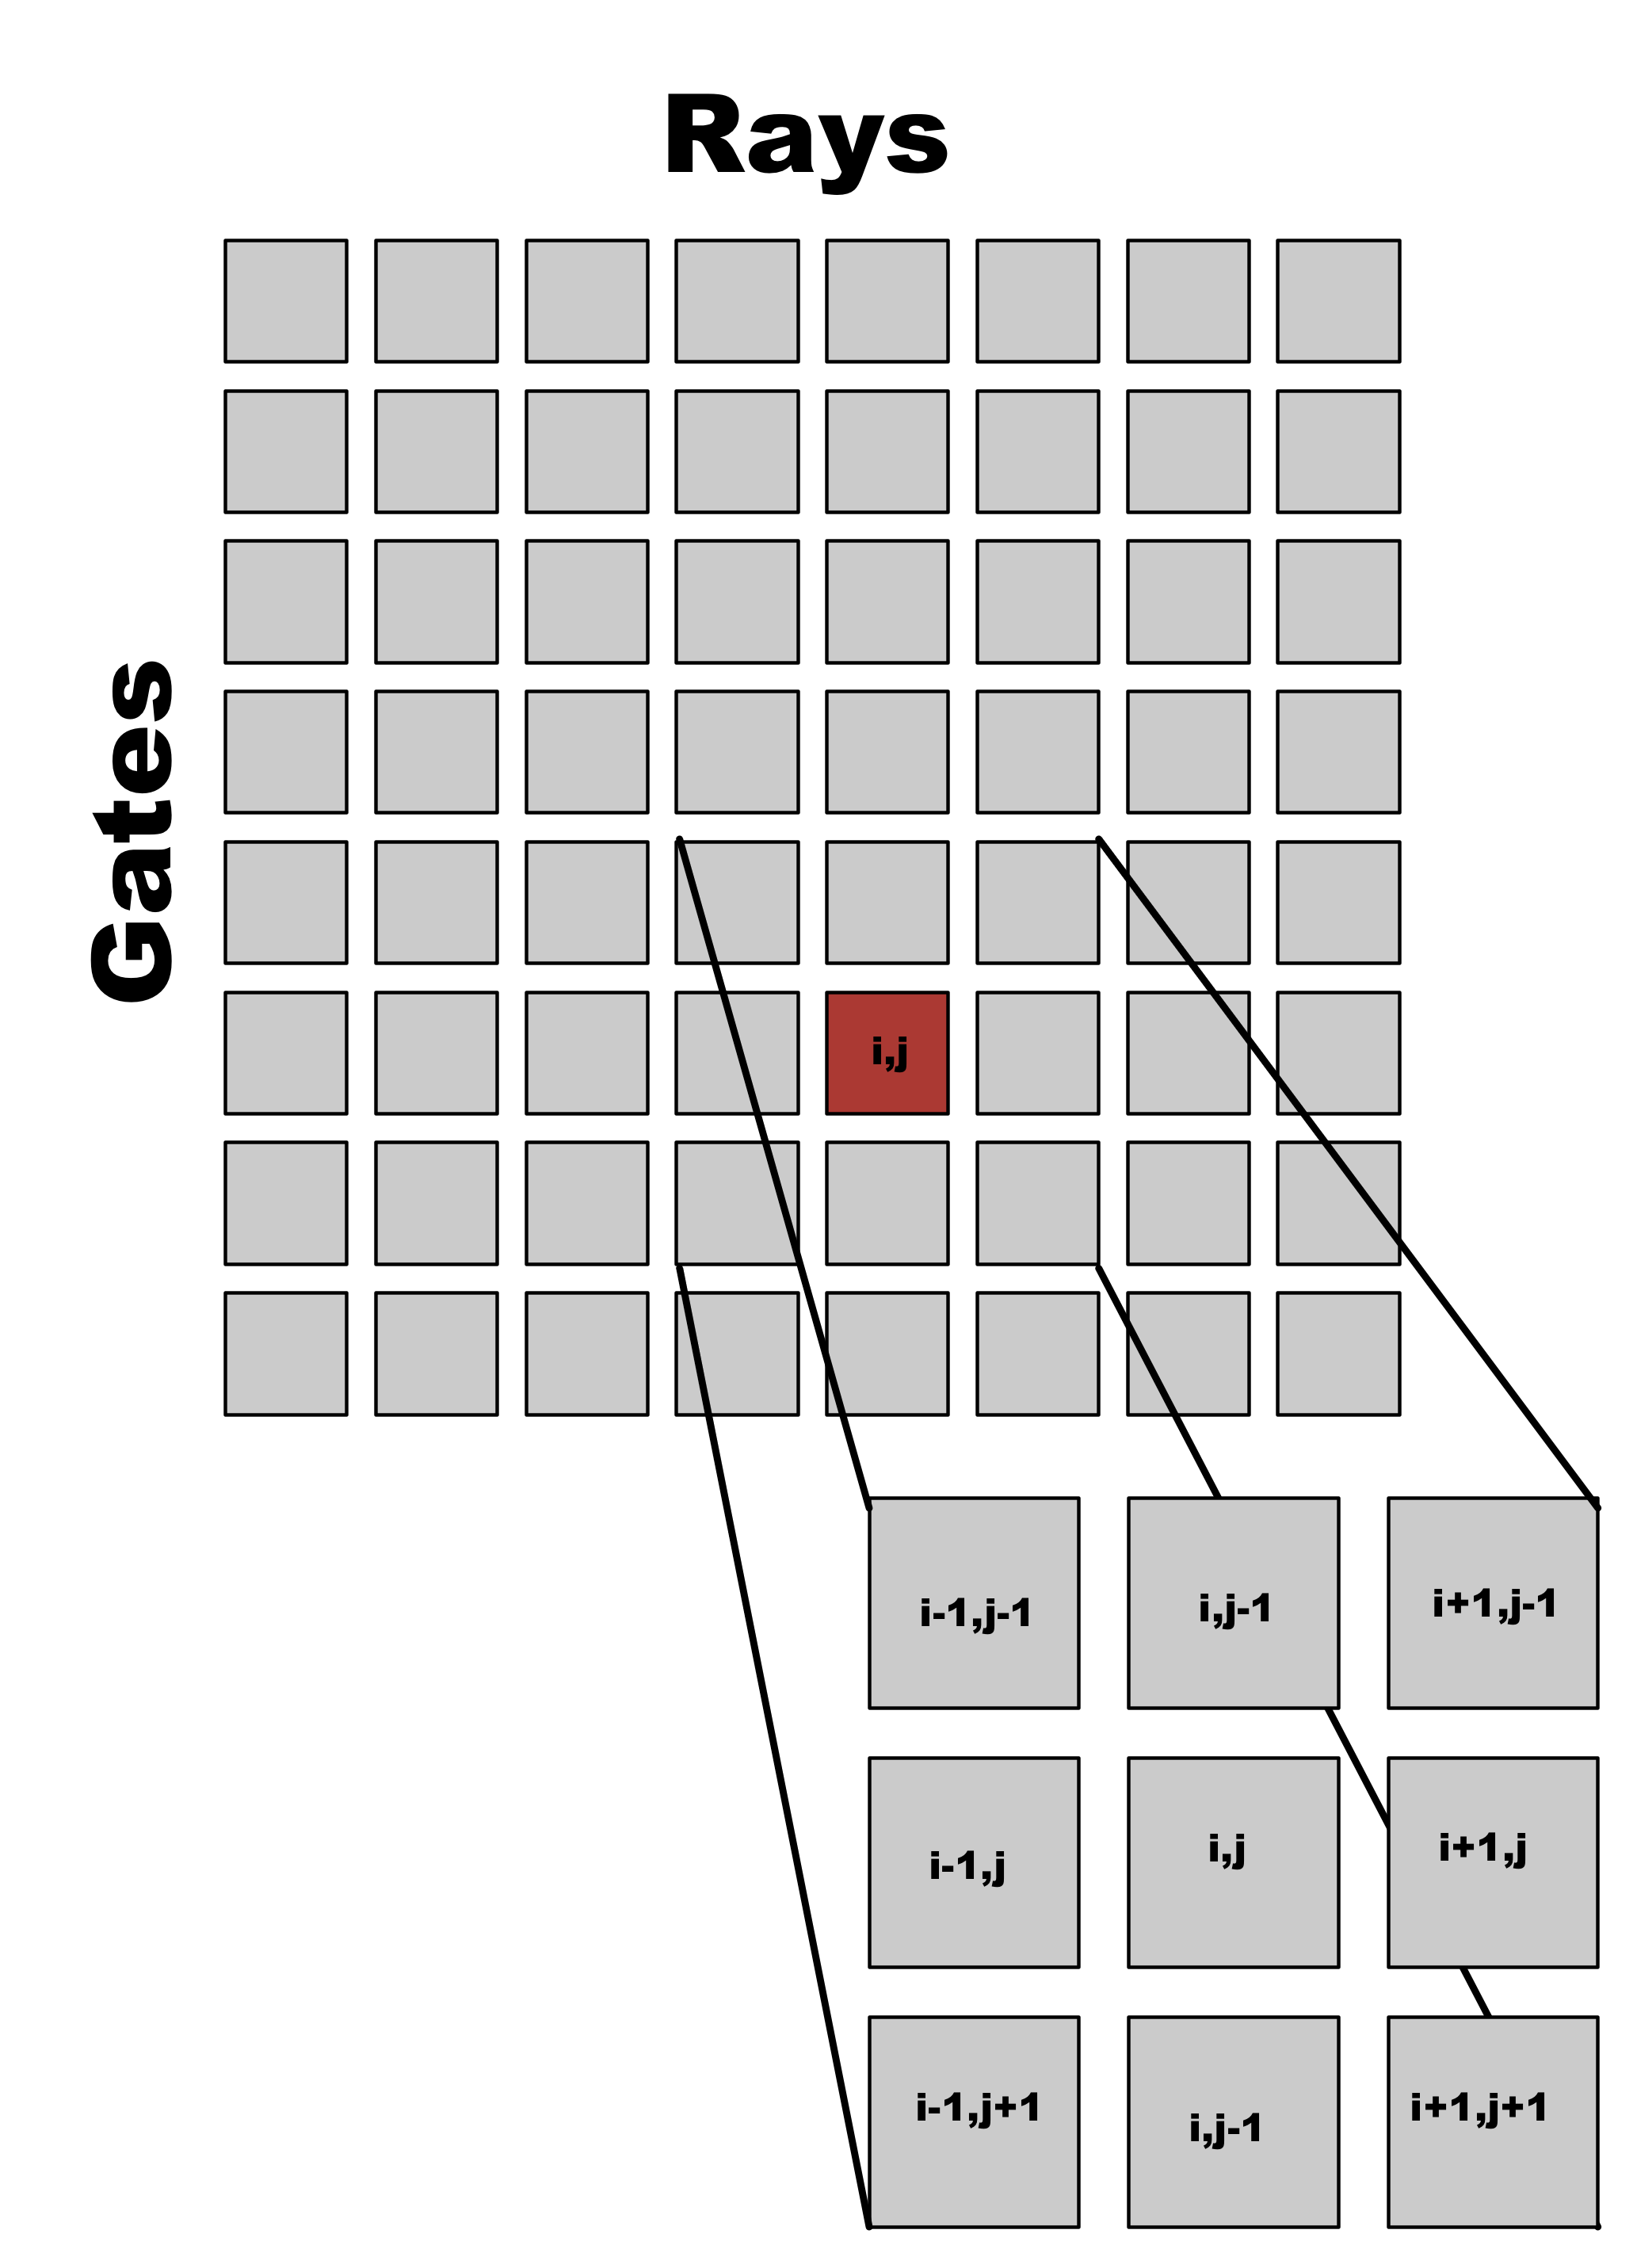
\includegraphics[width=0.8\columnwidth]{grid.png}
    \caption{Illustration of the concept of a moving filter over range gates of adjacent rays. 
    The center element, $\mathrm{(i,j)}$ is calculated by passing surrounding elements. 
    The footprint of the surrounding elements is determined by the kernel. In many cases we use a 3x3 kernel}
    \label{fig:grid}
\end{figure}

The challenge comes from the desire to calculate this pre-correction. Doppler folding will generate a 
significant signal in the texture field if done purely on radial velocity values. However projection of radial 
velocity values onto a unit circle allows a smooth transition from positive nyquist to negative nyquist 
and there is a branch of mathematics dealing with the statistics of directions and magnitudes known
 as directional statistics (\cite{wiki:dstats}). Values from positive nyquist to negative nyquist are projected
  onto a circle with $\theta$ = 0 to $\mathrm{\pi}$ and the standard deviation is given by:

\begin{align}
x &= \cos{\theta}\\
y &= \sin{\theta}\\
R &= \sqrt{\bar{x}^2 + \bar{y}^2}\\ 
S &= \sqrt{-2 * \log{R}}
\label{eq:tex}
\end{align}

Figure \ref{fig:textcalc:vr} shows a typical radial velocity field, with folds, from the ARM C-SAPR at the Southern Great Plains. Figure \ref{fig:textcalc:tx} shows the texture field calculated by passing eq. \ref{eq:tex} over data in \ref{fig:textcalc:vr} using a 3x3 kernel as shown in fig \ref{fig:grid}. 

\begin{figure}[h]
    \centering
    \begin{subfigure}[b]{0.4\columnwidth}
        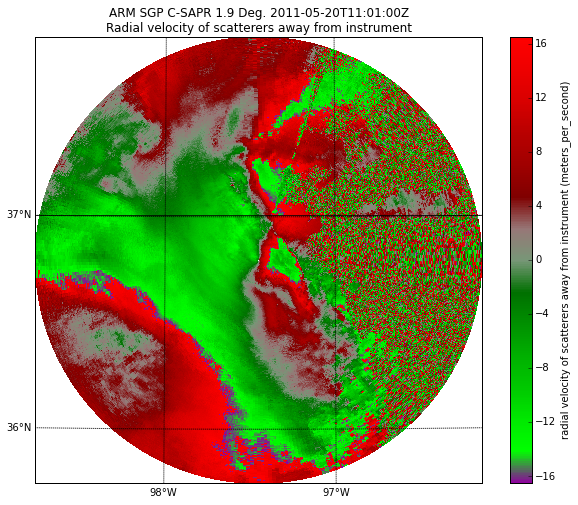
\includegraphics[width=\columnwidth]{radial_velocity.png}
        \caption{Radial velocity}
        \label{fig:textcalc:vr}
    \end{subfigure}
     %add desired spacing between images, e. g. ~, \quad, \qquad, \hfill etc. 
      %(or a blank line to force the subfigure onto a new line)
    \begin{subfigure}[b]{0.4\columnwidth}
        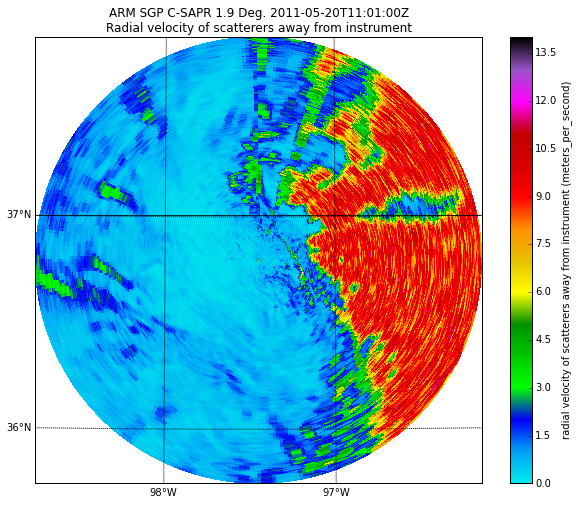
\includegraphics[width=\columnwidth]{texture.png}
        \caption{Texture}
        \label{fig:textcalc:tx}
    \end{subfigure}
    \caption{Calculations of texture of radial velocity from the C-Band Scanning ARM Precipitation Radar (C-SAPR) using circular statistic to avoid false texture on folds}
\end{figure}

There are clearly higher values of texture where there are no significant returns while texture falls 
quickly over the precipitation echo boundaries. However the exact values of texture to be used 
in the membership function to delineate between significant and non-significant will depend on 
many factors that influence texture including number of samples, signal to noise etcetera.
 Plotting a histogram of texture values yields  two distinctly separated populations of gates. 
 To find the discrimination point we use Scientific Python's (\cite{scipy}) continuous wavelet transform-based
 peak finding algorithm (\cite{Du01092006}) to find the location of the left and right peak. The cut off is then
 decided by finding the minimum value, or valley, between the two peaks. Ad-hoc testing shows this to be robust
 even when changing radar types. We tested with X,C and Ka band radars all using different configurations. 
 

\begin{figure}[h]
    \centering
    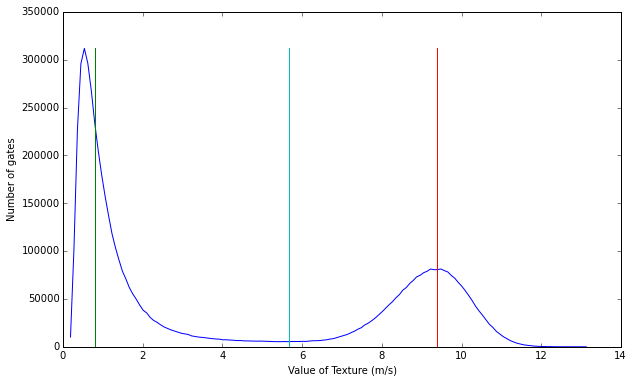
\includegraphics[width=0.95\columnwidth]{peak_finding.png}
    \caption{Histogram of texture values from the volume shown in fig \ref{fig:textcalc:vr}. The left hand peak corresponds to 
    significant returns, the right hand to noise. The black and red lines are the peak center guess by a wavelet based technique. 
    The green line is the minimum value between the two peaks. }
    \label{fig:grid}
\end{figure}


\subsection{Fuzzy logic based identification of scatterers at gate}
As previously discussed the aim of this step is to identify the dominant scatterer at each gate to aid in decision making 
upchain. Work has been done using fuzzy logic for precipitation determination before (see, for example
  \cite{gourley_fuzzy_2007}). However since ARM is not doing 



\begin{table*}[ht]
\caption{Wide single-column table in a twocolumn document.}
\centering
\begin{tabular}{p{0.05\linewidth}p{0.12\linewidth}p{0.16\linewidth}p{0.12\linewidth}p{0.14\linewidth}p{0.12\linewidth}p{0.14\linewidth}}
\hline
Class & Tex (m/s)& $\rho_{HV} $ &NCP & Temperature (C) &height (km)  & SNR (dB)\\
\hline
melting & [0, 0, 4, 6], 1.5& [0.6, 0.65, 0.9, 0.96], 3.5& [0.4, 0.5, 1, 1], 0& [0, 0.5, 6, 7], 1& [0, 0, 25, 25], 0& [8, 10, 1000, 1000], 0 \\
multi trip &[5, 6, 130, 130], 5&[0.5, 0.7, 1, 1], 0&[0, 0, 0.5, 0.6], 0&[-100, -100, 100, 100], 0&[0, 0, 5, 8], 0&[15, 20, 1000, 1000], 1\\
rain &[0, 0, 4, 6], 1& [0.97, 0.98, 1, 1],1.0& [0.4, 0.5, 1, 1], 1& [2, 5, 100, 100], 2& [0, 0, 5, 6], 0]& [8, 10, 1000, 1000], 1\\
snow &[0, 0, 4, 6], 1& [0.65, 0.9, 1, 1],1.0& [0.4, 0.5, 1, 1], 1& [-100, -100, 0.5, 4.0], 2& [0, 0, 25, 25], 0& [8, 10, 1000, 1000], 1\\
\hline
\end{tabular}
\end{table*}


%\begin{table*}
%\centering
%\begin{tabular*}{lcr}
%1 & 2 & 3 \        4 & 5 & 6 \        7 & 8 & 9
%%\topline
%%Class & Tex& $\rho_{HV}$ &NCP & height & Temperature & SNR\\
%%1 & 2 & 3 & 4 & 5& 6\
%%\midline
%%[[5.,6.,130.,130.], 5.0] & [[.5,.7,1,1], 0.0] & [[0,0,.5,.6], 0.0] & [[0,0,5000,8000], 0.0] & [[-100,-100,100,100], 0.0] & [[15,20, 1000,1000],1.0] \
%%\botline
%\end{tabular*}
%\end{table*}

\section{Challeges}
The data u

\section{Future work}
The climatology and varianc

%%%%%%%%%%%%%%%%%
%ACKNOWLEDGMENTS
%%%%%%%%%%%%%%%%%

\acknowledgments{}

Scott G

Patricia

%%%%%%%%%%%%%%%%%
%APPENDIXES
%%%%%%%%%%%%%%%%%
%\appendix
%\appendixtitle{Appendix Title}
%
%\subsection*{Appendix section head}
%
%Here is a sample appendix.
%\begin{equation}
%\frac{
%pf \cos\phi}
%{p^0|\nabla h\bar q|(d\theta_0/dz)}
%\end{equation}
%
%\appendix[B]
%\appendixtitle{Second Appendix Title}
%\subsection{Sample appendix section head}
%Second appendix example.
%\subsection{Sample appendix section head}
%\begin{equation}
%\left(\frac{\partial\bar q}{\partial x}
%\overline{U'\theta'} +
%\frac{\partial\bar q}{\partial y}
%\overline{V'\theta'}\right) 
%\end{equation}


%%%%%%%%%%%%%%%%%
%REFERENCES
%%%%%%%%%%%%%%%%%

\bibliographystyle{ametsoc2014}
\bibliography{zotero}

%%%%%%%%%%%%%%%%%
% TABLES
%%%%%%%%%%%%%%%%%

%\begin{table}
%\caption{Percentage of variance explained by the first four
%EOFs for the North Pacific Bx. The degree of separation between
%EOF1 and EOF2 and EOF2 and EOF3, based on the North et al.
%(1982) criterion, is indicated by good (GD) and not good or marginal
%(NG).}
%\begin{tabular*}{\hsize}{@{\extracolsep\fill}lcccccc@{}}
%\topline
%Month& EOF1& Split &EOF2& Split& EOF3& EOF4\\
%\midline
%\ Jan& 29& NG& 24& GD& 10& 5\\
%\ Feb& 39& GD& 20& GD& \phantom{1}7 &6\\
%\ Mar& 31& GD& 14& NG& 10& 6\\
%\ Apr& 23& GD& 14& NG& 10& 7\\
%\ May& 19& GD& 12& NG& 10& 7\\
%\ Jun& 19& GD& 12& NG& 10& 9\\
%\ Jul& 18& NG &13& NG& \phantom{1}9& 7\\
%\ Aug& 18& NG& 13& NG& 11& 9\\
%\ Sep &17& NG& 13& NG& 10& 8\\
%\ Oct &16& NG& 13& GD& \phantom{1}8& 7\\
%\ Nov &19 &NG& 16& NG& 11& 8\\
%\ Dec& 33& GD& 18& GD& 10& 6\\
%\botline
%\end{tabular*}
%\end{table}

%
%
%\begin{table}
%\centering
%\caption{Years selected for anomaly composites for the positive
%phase of $B^x$ EOF1.}
%\begin{tabular}{lc}
%\topline
%Month& Yr of positive phase\\
%\midline
%\ \ Jan& 1961, 1969, 1978, 1979, 1988, 1990, 1992, 1994\\
%\ \ Feb& 1964, 1977, 1978, 1980, 1983, 1986, 1988, 2000, 2001\\
%\ \ Mar& 1970, 1973, 1979, 1980, 1984, 1988, 2000\\
%\ \ Apr& 1959, 1961, 1962, 1963, 1968, 1972, 1983, 2002\\
%\ \ May& 1971, 1984, 1993, 1996, 2000\\
%\ \ Jun& 1981, 1983, 1984, 1993, 1998\\
%\ \ Jul& 1961, 1972, 1973, 1978, 1994, 2000\\
%\ \ Aug& 1967, 1970, 1973, 1978, 1994, 1999\\
%\ \ Sep& 1975, 1977, 1988, 1989, 1994, 1998, 1999\\
%\ \ Oct& 1962, 1977, 1998, 1999, 2001\\
%\ \ Nov& 1985, 1986, 1987, 1988, 1991, 1998\\
%\ \ Dec& 1957, 1968, 1972, 1978, 1979, 1990\\
%\botline
%\end{tabular}
%\end{table}
%
%\begin{table}
%\centering
%\caption{Years selected for anomaly composites for the negative
%phase of $B^x$ EOF1.}
%\begin{tabular}{lc}
%\topline
%Month& Yr of negative phase\\
%\midline
%\ \ Jan&1962, 1963, 1968, 1974, 1991, 1996, 1997\\
%\ \ Feb& 1959, 1963, 1971, 1974, 1976, 1979, 1985, 1989, 1990, 1994\\
%\ \ Mar& 1963, 1968, 1972\\
%\ \ Apr& 1984, 1988, 1993, 1996, 1999, 2000\\
%\ \ May& 1961, 1963, 1983, 1987, 1997\\
%\ \ Jun& 1961, 1972, 1978, 1980, 1982, 1986\\
%\ \ Jul& 1964, 1974, 1980, 1983, 1986, 1988, 1993\\
%\ \ Aug& 1980, 1987, 1991, 1993, 1997\\
%\ \ Sep& 1959, 1963, 1969, 1983, 1985, 1993\\
%\ \ Oct& 1957, 1986, 1993, 1996, 1997\\
%\ \ Nov& 1958, 1968, 1970, 1982, 1997\\
%\ \ Dec& 1969, 1974, 1976, 1985, 1998, 1999, 2000, 2001\\
%\botline
%\end{tabular}
%\end{table}

%%%%%%%%%%%%%%%%%
% FIGURES
%%%%%%%%%%%%%%%%%

%\begin{figure}[t]
%\centerline{\includegraphics[width=\textwidth]{figone.pdf}}
%
%\caption{Climatology of $Bx (10^{-6} s^{-1}$, color) and $U^{200}$(m s$^-1$,
%contours) for (a) February and (b) August; $\overline{V'\theta'}^{850}$
%(K m s$^-1$, color) and 
%$\overline{V'V'}^{200}$
%(m$^2$ s$^{-1}$, contours) for (c) February and (d) August; MR$^{z850}$ 
%(10$^{-3}$ m$^2$ s$-2$, color) and $U^{1000}$ (m s$^{-1}$, contours) 
%for (e) February and (f) August;
%and SST (K, color) and $F_h$ [10$^5$ J m$^{-2}$ (6 h)$^{-1}$] for (g)
%February and (h) August. Red rectangles indicate the domain of EOF
%calculations.} \label{fig1} 
%\end{figure}
%
%\begin{figure}[p]
%\centerline{\includegraphics{FigTwo.pdf}}
%\caption{As in Fig.~10, but for (a),(b) September EOF1; (c),(d) September EOF2; (e),(f) October EOF1; (g),(h) October EOF2; and
%(i),(j) December EOF2.}
%\end{figure}
%
%\begin{figure}
% \centerline{\includegraphics[width=19pc]{figure01.pdf}}
%\appendcaption{A1}{Here is an appendix, single column figure caption.}
%\end{figure}
%



\end{document}





